\documentclass[a4paper,14pt]{extarticle}

\usepackage{cmap}
\usepackage[T2A]{fontenc}
\usepackage[utf8x]{inputenc}
\usepackage[english, russian]{babel}

\usepackage{misccorr} % в заголовках появляется точка, но при ссылке на них ее нет
\usepackage{amssymb,amsfonts,amsmath,amsthm}  
\usepackage{indentfirst}
\usepackage[usenames,dvipsnames]{color} 
\usepackage[unicode,hidelinks]{hyperref}
% \hypersetup{%
%     pdfborder = {0 0 0}
% }

\usepackage{makecell,multirow} 
\usepackage{ulem}
\usepackage{graphicx,wrapfig}
\graphicspath{{img/}}
\usepackage{geometry}
\geometry{left=2cm,right=2cm,top=3cm,bottom=3cm,bindingoffset=0cm,headheight=15pt}
\usepackage{fancyhdr} 
\linespread{1.05} 
\frenchspacing 
\renewcommand{\labelenumii}{\theenumii)} 
\newcommand{\mean}[1]{\langle#1\rangle}
% \usepackage{caption}
%%%%%%%%%%%%%%%%%%%%%%%%%%%%%%%%%%%%%%%%%%%%%%%%%%%%%%%%%%%%%%%%%%%%%%%%%%%%%%%
%%%%%%%%%%%%%%%%%%%%%%%%%%%%%%%%%%%%%%%%%%%%%%%%%%%%%%%%%%%%%%%%%%%%%%%%%%%%%%%

\def\labauthors{Сарафанов Ф.Г., Платонова М.В.}
\def\labgroup{430}
% \def\department{Кафедра электроники и квантовой физики}
\def\labnumber{2}
\def\labtheme{}

%%%%%%%%%%%%%%%%%%%%%%%%%%%%%%%%%%%%%%%%%%%%%%%%%%%%%%%%%%%%%%%%%%%%%%%%%%%%%%%
	%применим колонтитул к стилю страницы
\pagestyle{fancy} 
	%очистим "шапку" страницы
\fancyhead{} 
	%слева сверху на четных и справа на нечетных
\fancyhead[L]{\labauthors} 
	%справа сверху на четных и слева на нечетных
\fancyhead[R]{КНД рупорной антенны} 
	%очистим "подвал" страницы
\fancyfoot{} 
	% номер страницы в нижнем колинтуле в центре
\fancyfoot[C]{\thepage} 
\renewcommand{\phi}{\varphi}
%%%%%%%%%%%%%%%%%%%%%%%%%%%%%%%%%%%%%%%%%%%%%%%%%%%%%%%%%%%%%%%%%%%%%%%%%%%%%%%

\usepackage{float}
\usepackage[mode=buildnew]{standalone}
\usepackage{tikz} 
% \usepackage{subcaption}
\usepackage{tikz,csvsimple}
\usetikzlibrary{scopes}
\usetikzlibrary{%
     decorations.pathreplacing,%
     decorations.pathmorphing,%
    patterns,%
    calc,%
    scopes,%
    arrows,%
    % arrows.spaced,%
}
\makeatletter
\newif\if@gather@prefix 
\preto\place@tag@gather{% 
  \if@gather@prefix\iftagsleft@ 
    \kern-\gdisplaywidth@ 
    \rlap{\gather@prefix}% 
    \kern\gdisplaywidth@ 
  \fi\fi 
} 
\appto\place@tag@gather{% 
  \if@gather@prefix\iftagsleft@\else 
    \kern-\displaywidth 
    \rlap{\gather@prefix}% 
    \kern\displaywidth 
  \fi\fi 
  \global\@gather@prefixfalse 
} 
\preto\place@tag{% 
  \if@gather@prefix\iftagsleft@ 
    \kern-\gdisplaywidth@ 
    \rlap{\gather@prefix}% 
    \kern\displaywidth@ 
  \fi\fi 
} 
\appto\place@tag{% 
  \if@gather@prefix\iftagsleft@\else 
    \kern-\displaywidth 
    \rlap{\gather@prefix}% 
    \kern\displaywidth 
  \fi\fi 
  \global\@gather@prefixfalse 
} 
\newcommand*{\beforetext}[1]{% 
  \ifmeasuring@\else
  \gdef\gather@prefix{#1}% 
  \global\@gather@prefixtrue 
  \fi
} 
\makeatother

\usepackage{booktabs}
\usepackage{pgfplots, pgfplotstable}

\usepackage[outline]{contour}
\usepackage{tocloft}
\renewcommand{\cftsecleader}{\cftdotfill{\cftdotsep}} % for parts
% \renewcommand{\cftchapleader}{\cftdotfill{\cftdotsep}} % for chapters
\usepackage{pgfplots,pgfplotstable,booktabs,colortbl}
\pgfplotsset{compat=newest}
\usepackage{physics}
\usepackage{mathtools}
\mathtoolsset{showonlyrefs=true}
\newcommand\Smat{\hat { \mathbf { S } }}

\newcommand*\dotvec[1][1,1]{\crossproducttemp#1\relax}
\def\crossproducttemp#1,#2\relax{{\qty[\vec{#1}\times\vec{#2}\,]}}

\newcommand*\prodvec[1][1,1]{\crossproducttempa#1\relax}
\def\crossproducttempa#1,#2\relax{{\qty[{#1}\times{#2}\,]}}

% \def\E{\mathscr{E}_H}
\def\Rdim{\,\frac{\text{м}^3}{\text{А} \cdot \text{с}}}

\renewcommand{\vec}{\mathbf} % for parts

\begin{document}
\begin{titlepage}
\begin{center}
% \vspace{-3em}
{\small\textsc{Нижегородский государственный университет имени Н.\,И. Лобачевского}}
\vskip 2pt \hrule \vskip 3pt
{\small\textsc{Радиофизический факультет}}

\vfill


{{\large Отчет по лабораторной работе №\labnumber}\vskip 12pt {\LARGE \bfseries Определение КНД \\[0.2em] рупорной антенны}}

	
\vspace{2cm}
{\large Работу выполнили студенты \\[-0.25em] 440 группы радиофизического факультата \\[0.5em] {\Large \bfseries \labauthors}}

% \vspace{0.5cm}
% {e-mail: sfg180@yandex.ru}

% \vspace{2cm}

\end{center}

\vfill
	
% \begin{flushright}
% 	{Выполнили студенты 430 группы\\ \labauthor}%\vskip 12pt Принял:\\ Менсов С.\,Н.}
% \end{flushright}
	
% \vfill
	
\begin{center}
	{Нижний Новгород, 24 сентября -- \today}
\end{center}

\end{titlepage}
\tableofcontents
\newpage


% \section{Теоретическая часть}

\addcontentsline{toc}{section}{Введение}
\section*{Введение}

В настоящей работе определяется коэффициент направленного действия (сокращенно -- КНД) пирамидальной рупорной антенны с помощью зеркального метода. КНД характеризует выигрыш по мощности в направлении максимального излучения вследствие направленности антенны.

\paragraph{Установка.} СВЧ-излучение, созданное генератором клистронного типа, через волноводный тракт с измерительной линией подается на рупорную антенну. При этом длина излучаемой волны $\lambda \sim 3$ см.

Рупорная антенна и волноводный тракт находятся на платформе, положение оной относительно щита регулируется винтовой передачей. Установка работает в несогласованном режиме, что приводит к появлению отраженной от конца подводящего тракта волны.

Все измерения базируются на получении интенсивности поля внутри волновода при определенном положении квадратичного детектора относительно измерительной линии (которое также регулируется винтовой передачей). При измерениях снимаются показания амперметра, подключенного к детектору.

\paragraph{Зеркальный метод.} Для реализации зеркального метода используется два щита: поглощающий и отражающий, которые выставляются параллельно излучающей апертуре рупорной антенны.

Выставление щитов позволяет провести отдельные измерения при наличии и отсутствии отраженного сигнала.

Измерение интенсивности поля внутри волновода также позволяет получить длину волны в волноводе, максимальные и минимальные значения интенсивности. На основании таких измерений, как будет показано далее, можно найти коэффициент направленного действия $D$. 

Все измерения проводятся таким образом, чтобы отражающий экран находился в зоне Фраунгофера, т.е. там, где сформирована диаграмма направленности антенны.

\newpage

\section{Расчет для измерения КНД}

Воспользуемся методом изображений для получения отраженного от щита поля. Для этого представим отраженное поле как созданное такой же антенной, зеркально расположенной относительно щита.

Мощность на единицу телесного угла, излучаемая мнимой антенной в направлении реальной, в силу определения $D=4\pi\frac{P_\text{пад}}{P_\text{изл}}$ равна
\begin{equation}
  P_\text{пад}=D\frac{P_\text{изл}}{4\pi},
\end{equation}
отсюда плотность потока энергии в месте приема, в силу определения $P=r^2 S_r$,
\begin{equation}
  S_\text{пад}=\frac{P_n}{4X^2}=D\frac{P_\text{изл}}{16\pi X^2}.
\end{equation}

Так как КНД плоской антенны $D$ связано с эффективной площадью плоской антенны $A=\frac{P_\text{прин}}{S_\text{пад}}$ соотношением
\begin{equation}
  A=\frac{\lambda^2}{4\pi}D,
\end{equation}
то отсюда окончательно получаем
\begin{equation}
    \frac{P_\text{прин}}{P_{\text{изл}}} = \frac{D^2\lambda^2}{64\pi^2X^2},
\end{equation}
и тогда интересующая нас величина $D$ представляется в виде 
\begin{equation}
    D = \frac{8\pi X}{\lambda}\sqrt{\frac{P_\text{прин}}{P_\text{изл}}} = \frac{8 \pi X}{\lambda} \Gamma.
    \label{eq:DG}
\end{equation}

Таким образом, экспериментальное определение КНД требует нахождения отношения принимаемой зеркально отраженной мощности к мощности, излучаемой пирамидальной рупорной антенной. 


Запишем значение поля, отнормированное на амплитуду падающей волны, для некоторого фиксированного положения рупора:
\begin{equation}
    E = 1e^{-ihx}+\Gamma_\kappa e^{i\varphi_\kappa} e^{ihx}+ \Gamma e^{e\varphi} e^{ihx}.
    \label{eq:11}
\end{equation}
Смещение антенны на величину $\Delta X$ приведет к появлению в последнем члене дополнительного множителя $e^{i k_0 2\Delta X }$, связанного с дополнительным набегом фазы в свободном пространстве. 
Поскольку 
$ \Gamma_{\kappa}$ и  $\Gamma$ достаточно малы, то квадратичными величинами в первом приближении можно 
пренебречь. В результате для $ |E|^2 $ будем иметь 
\begin{equation}
    |E|^{2} \approx 1+2 \Gamma_{\kappa} \cos \left(2 h x+\varphi_{\kappa}\right)+2 \Gamma \cos \left(2 h x+\varphi+k_{0} 2 \Delta X\right).
    \label{eq:13}
\end{equation}

Найдя экспериментально $\Gamma$, автоматически будет получено искомое значение $D$ по формуле \eqref{eq:DG}.


\section{Теоретическое значение КНД}

% Апертура рупора $l_1\times l_2 = 9.5 \text{ см} \times 14\text{ см}$, апертура волновода $ 1.02  \text{ см} \times 2.29 \text{ см}.$

Воспользуемся интегралом Френеля-Кирхгофа для нахождения компоненты поля:
\begin{equation}
  U(\mathbf{P})=\frac{ik}{2\pi z}e^{-ikz}\iint\limits_{\Sigma}U_0(x_0,y_0)\exp \Bigl\{-\frac{ik}{2z}\qty[(x-x_0)^2+(y-y_0^2)]\Bigr\}\dd x \dd y.
  \label{eq:fren}
\end{equation}
Здесь $\mathbf{P}(x,y,z)$ -- точка наблюдения, $\Sigma$ -- поверхность излучающей апертуры антенны.

Воспользуемся несколькими предположениями. Во-первых, точка наблюдения находится в зоне Фраунгофера, тогда $$\exp[-\frac{ik}{2z}(x_0^2+y_0^2)]\approx 1.$$ Во-вторых, рассмотрим малоугловое приближение (найдем поле вблизи оси, т.е. положения максимума излучения), тогда $$\exp \Bigl[-\frac{ik}{2z}(x^2+y^2)\Bigr]\approx 1.$$ Наконец, сделаем предположение об синфазности поля на излучающей апертуре, тогда \eqref{eq:fren} перейдет к виду
\begin{equation}
    U(\mathbf{P}) = U_0\frac{ e^{-i k z} }{i \lambda z} \iint\limits_{\Sigma}\exp[\frac{i k}{2 z}\qty(x^2+y^2)]\dd x \dd y.
    \label{eq:up1}
\end{equation}

При вычислении последнего выражения появятся интегралы Френеля, которые можно найти только численно. В первом приближении интегралы Френеля дают площадь апертуры, тогда
\begin{equation}
    U(\mathbf{P}) \sim U_0\cdot \Sigma \cdot \frac{e^{-i k z}}{i\lambda z}.
    \label{eq:up}
\end{equation}

Теперь можно найти КНД, последовательно выразив плотность потока энергии в максимуме и во всех направлениях (эквивалентного источника):
\begin{equation}
    S_{\max} = \frac{c}{8 \pi} \frac{U_0^2 \Sigma^2}{r^2 \lambda^2}, \quad S_{r} =\frac{1}{4 \pi } \frac{c}{8 \pi} \frac{U_0^2 \Sigma}{r^2 } 
    \label{eq:smsr}
\end{equation}
Тогда окончательно получаем выражение для КНД:
\begin{equation}
    D = \frac{S_{\max}}{S_r} = 4\pi\frac{\Sigma}{\lambda^2}
    \label{eq:kndt}
\end{equation}

В нашем случае апертура рупора $l_1\times l_2 = 9.5 \text{ см} \times 14\text{ см}$, т.е. $\Sigma = 133 \text{ см}^2$, а длина волны $\lambda \approx 3$ см, тогда 
\begin{equation}
  D\sim 180
\end{equation}
Следует критично воспринимать полученное значение КНД, так как оно получено при ряде предположений, каждое из которых понижает точность расчета. В частности, синфазность и однородность поля на излучающей апертуре, очевидно, не выполняются.

\newpage
\section{Экспериментальное определение КНД}
Перед измерением убедимся, что экран находится в зоне Фраунгофера:
\begin{equation}
    X = 274 \text{ см} \gg \frac{\max\{l_1^2,l_2^2\}}{\lambda} \sim 61 \text{ см}.
\end{equation}
\subsection{Поле при отсутствии принимаемого сигнала}
В этом эксперименте перед антенной был размещен поглощающий излучение щит, устраняющий отраженное от металлического щита поле, а в волноводе измерен ток детектора, пропорциональный интенсивности электрического поля $|E|^2$, в зависимости от координаты детектора в волноводе $x$ (см. рис. \ref{fig:exp:1}).

\begin{figure}[h!]
    \centering
    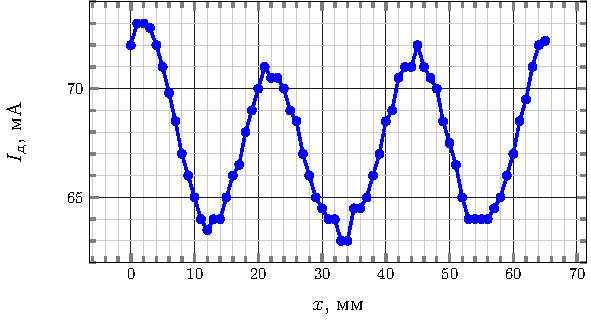
\includegraphics[scale=1.5]{fig/e2_from_x}
    \caption{Зависимость $I_\text{д}\sim|E|^2$ от координаты $x$}
    \label{fig:exp:1}
\end{figure}

В данном эксперименте, как нетрудно получить из \eqref{eq:13}, интенсивность зависит от координаты как
\begin{equation}
    |E|^2 \approx 1 + 2 \Gamma_{\kappa} \cos (2 h x + \varphi_{\kappa}) \quad \Rightarrow \quad
    |E_{\max}|^2=1+2\Gamma_\kappa, \quad
    |E_{\min}|^2=1-2\Gamma_\kappa,
    \label{eq:15}
\end{equation}
тогда
\begin{equation}
    \Gamma_{\kappa} = \frac{|E_{\max}|^2-|E_{\min}|^2}{2|E_{\max}|^2+2|E_{\min}|^2}=0.037
    \label{eq:16}
\end{equation}

Исходя из результатов эксперимента, можно найти длину волны в волноводе $\lambda_{\text{в}}$:
\begin{equation}
    \lambda_{\text{в}} \simeq 4.4 \text{ см}.
\end{equation}
Отсюда находится длина волны  в свободном пространстве $\lambda$:
\begin{equation}
    h^2 + \varkappa^2 = k^2  \Rightarrow \lambda = 
    \frac{2\pi}{
      \sqrt{
        \qty(\frac{2\pi}{\lambda_\text{в}})^2+
        \qty(\frac{\pi}{a})^2
      }
    } \simeq 3.06 \text{ см},  
    \label{eq:50}
\end{equation}
где $a = 2.29\text{ см}$ -- ширина волновода.

Оценим согласованность системы $\eta$:
\begin{equation}
  \eta \sim 1-\Gamma_\kappa^2 = 99.8\%
\end{equation}


\subsection{Поле при наличии принимаемого сигнала}
Найдя положение детектора $x = 7 \text{ мм}$, при котором $\cos (2 h x +\varphi_{\kappa} )=0$ и зафиксировав его, был убран поглощающий щит и снята зависимость $I_\text{д}\sim|E|^2(\Delta X)$, где $\Delta X$ -- смещение относительно металлического экрана. 
\begin{figure}[h!]
    \centering
    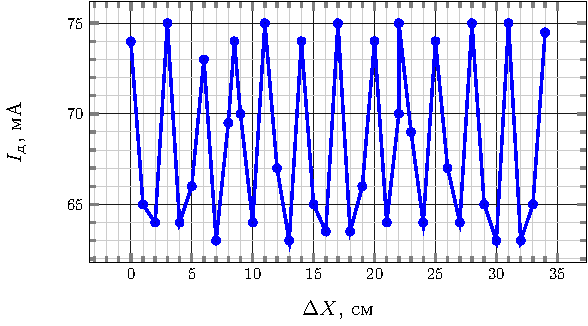
\includegraphics[scale=1.5]{fig/e2_from_dx}
    \caption{Зависимость $I_\text{д}\sim|E|^2$ от координаты смещения $\Delta X$}
    \label{fig:exp:2}
\end{figure}

После определения максимальных и минимальных значений на рис. \ref{fig:exp:2},  рассчитывается коэффициент отражения $\Gamma$:
\begin{equation}
    \Gamma = \frac{|E_{\max}|^2-|E_{\min}|^2}{2\qty( |E_{\max}|^2+|E_{\min}|^2 )} \approx 0.043
\end{equation}
Заметим, что положение антенны относительно щита $X=274$ см, тогда можем найти КНД:
\begin{equation}
    D = \Gamma \frac{8 \pi X}{\lambda} \simeq 98.04
\end{equation}




\subsection{Второй метод измерения КНД}
При изменении положения антенны  относительно отражающего щита $X +\Delta X$ были измерены $|E_{\max}|^2$ и $|E_{\min}|^2$ в измерительной линии. Из измерений можно выразить КБВ в линии $\kappa = E_{\min} / E_{\max}$, откуда рассчитать коэффициент $\tilde{\Gamma}$:
\begin{equation}
    \tilde{\Gamma}(\Delta X)= \frac{1-\kappa (\Delta X)}{1+\kappa (\Delta X)} = \frac{1-\sqrt{K(\Delta X)}}{1+\sqrt{K(\Delta X)}} 
\end{equation}
Полученная зависимость приведена на рис. \ref{fig:exp:3}.
\begin{figure}[h!]
    \centering
    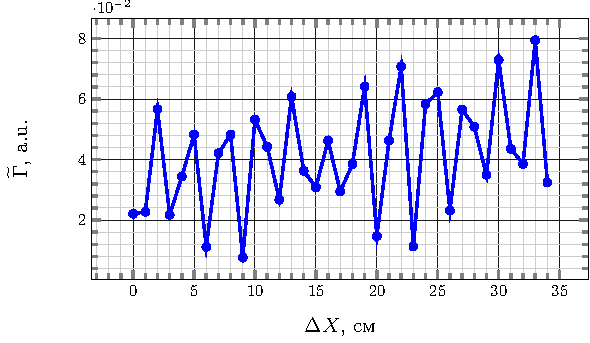
\includegraphics[scale=1.5]{fig/g_from_dx}
    \caption{Зависимость $\tilde{\Gamma}(\Delta X)$ }
    \label{fig:exp:3}
\end{figure}

Из найденного $\tilde{\Gamma}_{\max} \simeq 0.08$ можно найти значение $\Gamma \simeq \tilde{\Gamma}_{\max} -
\Gamma_{\kappa} \simeq 0.042$. Тогда можно выразить КНД: $$D \simeq 96.76$$ 

Обоснуем возможность применения формулы $\Gamma \simeq \tilde{\Gamma}_{\max} -
\Gamma_{\kappa}$. Для этого обратимся к формуле \eqref{eq:13}, откуда
\begin{equation}
    |E_{\min}|^{2} \approx 1-2 \Gamma_{\kappa}-2 \Gamma\cos \left(k_{0} 2 \Delta X\right), \quad
    |E_{\max}|^{2} \approx 1+2 \Gamma_{\kappa}+2 \Gamma\cos \left(k_{0} 2 \Delta X\right).
    \label{eq:eminmax}
\end{equation}
Максимальное значение $\tilde{\Gamma}$ достигается, очевидно, при наименьшем $K$, т.е. когда $\cos \left(k_{0} 2 \Delta X\right)=1$. Воспользуемся малостью $\Gamma$, $\Gamma_\kappa$ и разложим $\sqrt{K}$ в ряд по малому параметру $x=2\Gamma+2\Gamma_\kappa$:
\begin{equation}
  \sqrt{K}=\sqrt\frac{1-x}{1+x}\approx 1-x,
\end{equation}
тогда
\begin{equation}
  \tilde{\Gamma}_{\max}=\frac{1-(1-x)}{1+(1-x)}\approx \frac{x}{2} = \Gamma+\Gamma_\kappa.
\end{equation}


\addcontentsline{toc}{section}{Заключение}
\section*{Заключение}
В настоящей работе мы измерили КНД с помощью двух экспериментов $D_2=98.04$, $D_3=96.76$, а также при ряде приближений рассчитали теоретическое значение $D_1\sim 180$. Расхождение с практическими результатами объясняется неверным приближением синфазности поля на излучающей апертуре, что можно получить простым графическим построением моды TE${}_{10}$ с соблюдением условия $E_\tau=0$.

При начале измерений проверено соблюдение условия зоны Фраунгофера. Найдена длина волны в волноводе $\lambda_\text{в}=4.4$ см, в свободном пространстве $\lambda=3.06$ см. Проверена малость квадратичных величин $\Gamma_\kappa^2=1.3\cdot10^{-3}$, $\Gamma^2=1.8\cdot10^{-3}$, $\Gamma\cdot\Gamma_\kappa^2=1.5\cdot10^{-3}$, оценен КПД системы в смысле её согласованности $\eta=99.8\%$.

\begin{thebibliography}{}

  \bibitem{met1} Вайнштейн Л.А. Электромагнитные волны. М.: Радио и связь, 1988.

  \bibitem{lit3} Ландау Л.Д., Лифшиц Е.М. Теория поля. М.: Физматлит, 2003.
\end{thebibliography}

\end{document}